\subsection{Adding Customised Branching} \label{sbs:branch}
\begin{sloppypar}In \sbsref{sbs:callbacks} we explained the modifications made to \ac{DIP} and how a simple variable branch would be implemented.
The \ac{DIP} function \lstinline{chooseBranchSet} calls Dippy's \lstinline{branch_method} at fractional nodes.
The function \lstinline{branch_method} has two inputs supplied by \ac{DIP}:
\begin{enumerate}
\item \lstinline{prob} -- the \lstinline{DipProblem} being solved;
\item \lstinline{sol} -- an indexable object representing the solution at the current node.
\end{enumerate}
We define \lstinline{branch_method} using these inputs and the same PuLP structures used to defined the model, allowing Dippy to access the variables from the original formulation and eliminating any need for complicated indexing.\end{sloppypar}

We can explore custom branching rules that leverage constraints to reduce the symmetry in the solution space of the bin packing problem.
Inefficiencies arise from solvers considering multiple equivalent solutions that have identical objective function values and differ only in the subset of the identical bins used.
One way to address this is to add a constraint that determines the order in which the bins can be considered:
\[ y_i \geq y_{i+1}, i = 1, \ldots, m-1 \]
\lstinputlisting[firstnumber=61,linerange=61-62]{../../examples/Dippy/bpp/bin_pack_func.py}
This change results in a smaller branch-and-bound tree (see figure \ref{fig:bpp_tree2}) that provides the same solution but with bin 0 used in place of bin 3, i.e., a symmetric solution, but with the bins now used ``in order''.
\begin{figure}[htp]
\begin{center}
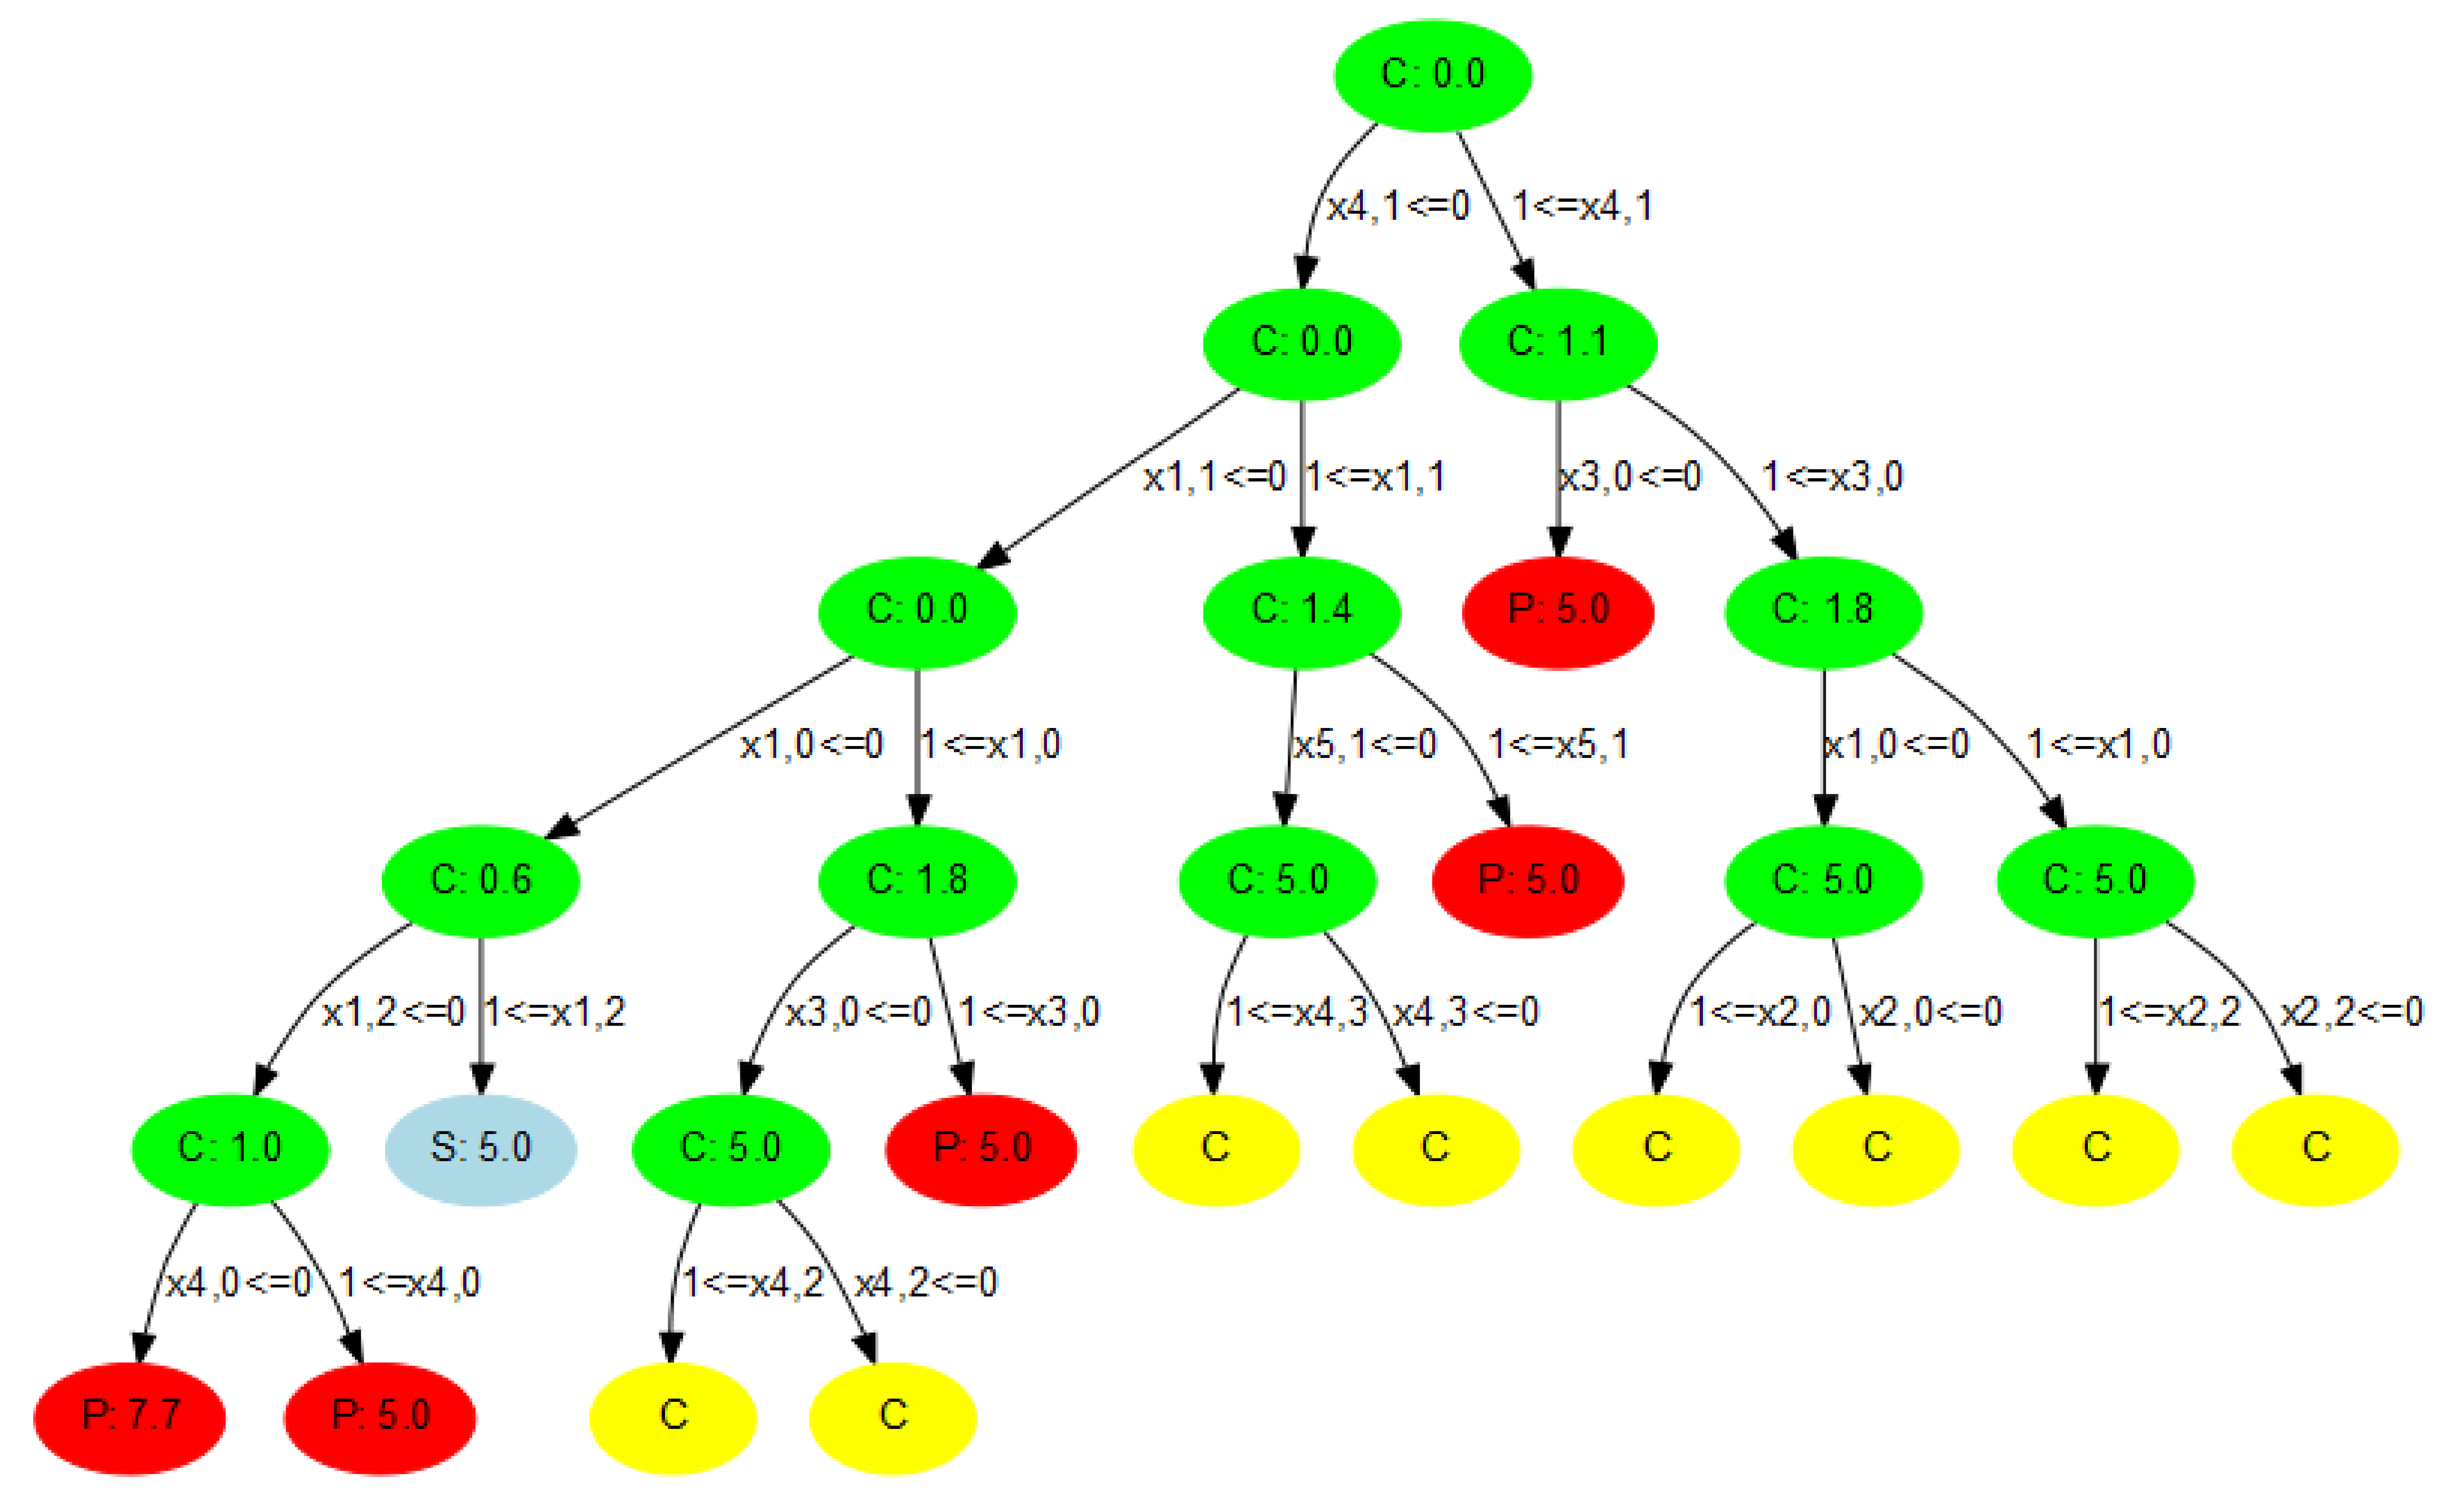
\includegraphics[scale=0.11]{img/bpp_tree2.eps}
\end{center}
\caption{Branch-and-bound tree for bin packing problem instance with anti-symmetry constraints.} \label{fig:bpp_tree2}
\end{figure}

These ordering constraints also introduce the opportunity to implement an effective branch on the number of facilities:

If $\displaystyle\sum_{i=1}^m y_i = \alpha \notin \mathbb{Z}$, then:
\vspace*{-6pt}
\begin{center}
\begin{tabular}{l|l}
the branch down restricts & the branch up restricts \\
$\displaystyle\sum_{i=1}^m y_i \leq \lfloor \alpha \rfloor$ &
$\displaystyle\sum_{i=1}^m y_i \geq \lceil \alpha \rceil$ \\
and the ordering means that & and the ordering means that \\
$y_i = 0, i = \lceil \alpha \rceil, \ldots, m$ &
$y_i = 1, i = 1, \ldots, \lceil \alpha \rceil$
\end{tabular}
\end{center}

\begin{sloppypar}We can implement this branch in Dippy by writing a definition for the \lstinline{branch_method}.\end{sloppypar}
\lstinputlisting[firstnumber=73,linerange={73-75,82-83}]{../../examples/Dippy/bpp/bin_pack_func.py}
\lstinputlisting[firstnumber=182,linerange={182-188,190-193,195-201,203-204,206-207}]{../../examples/Dippy/bpp/bin_pack_func.py}

The advanced branching decreases the size of the branch-and-bound tree further (see figure \ref{fig:bpp_tree3}) and provides another symmetric solution with the bins used in order.
\begin{figure}[htp]
\begin{center}
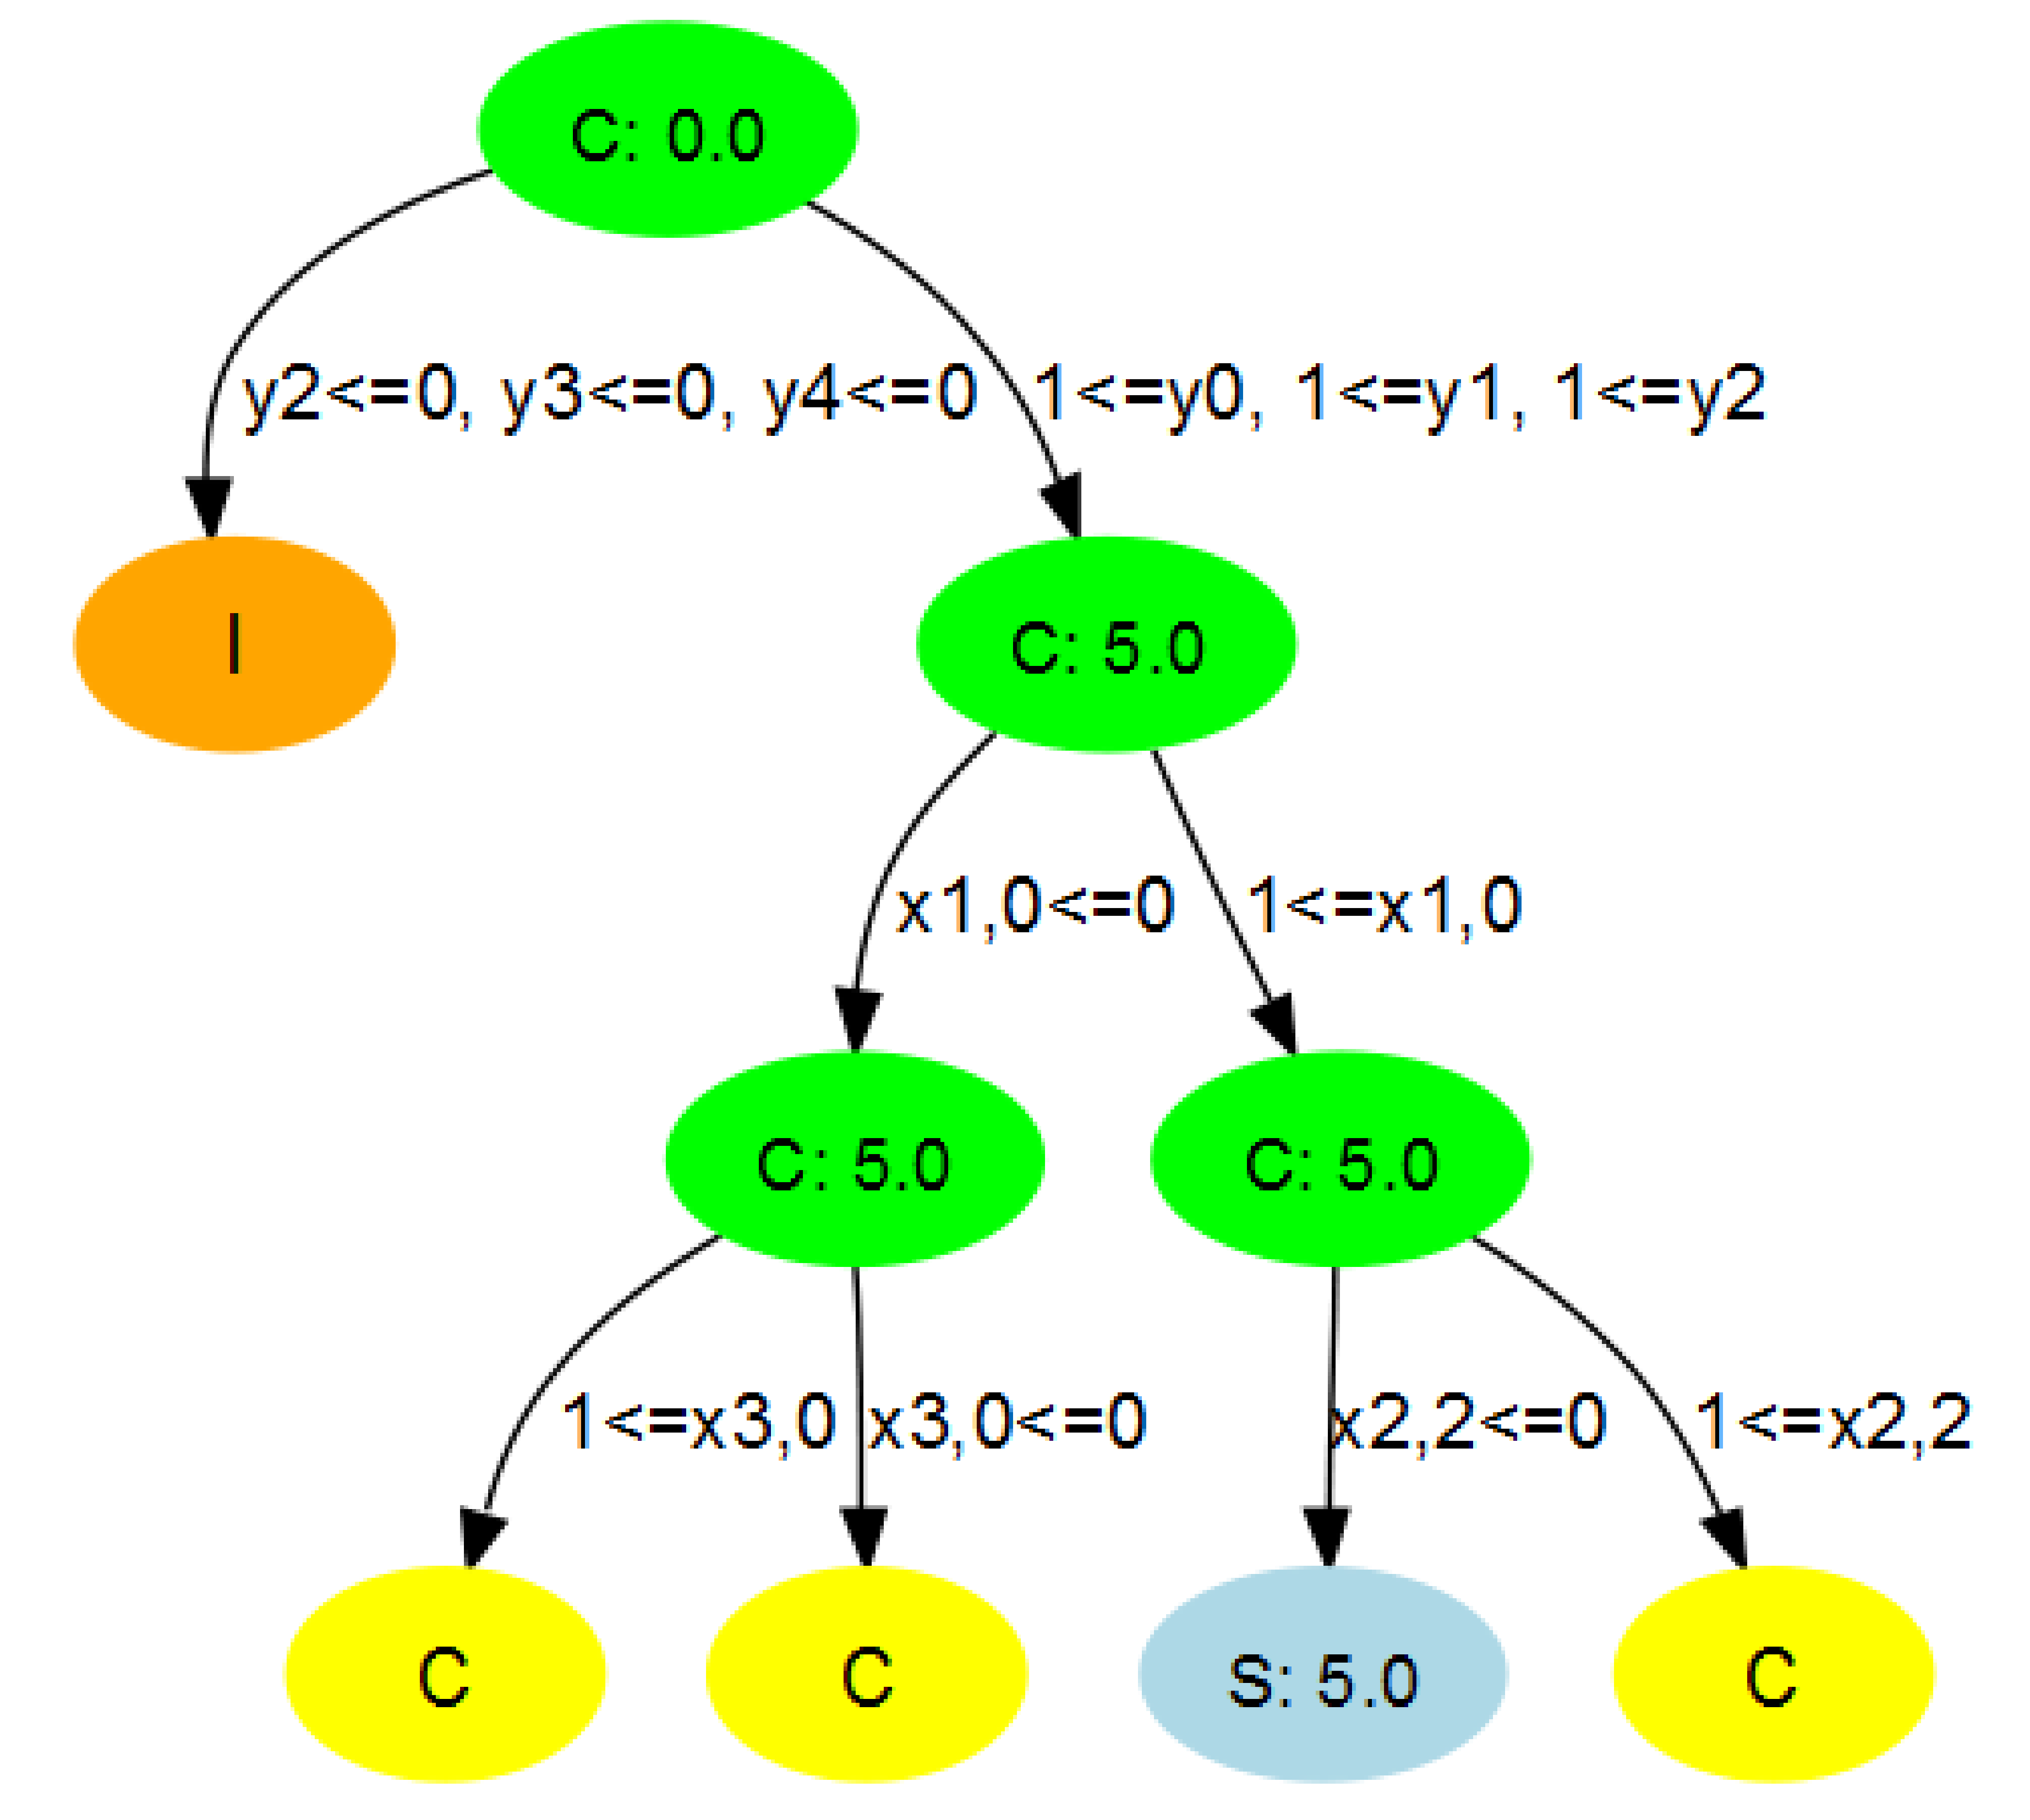
\includegraphics[scale=0.08]{img/bpp_tree3.eps}
\end{center}
\caption{Branch-and-bound tree for bin packing problem instance with anti-symmetry constraints and advanced branching.} \label{fig:bpp_tree3}
\end{figure}


\subsection{Adding Customised Cut Generation} \label{sbs:cuts}
To add user-defined cuts in Dippy, we first define a new procedure for generating cuts and (if necessary) a procedure for determining a feasible solution. Within Dippy, this requires two new functions, \texttt{generate\_cuts} and (if necessary) \texttt{is\_solution\_feasible}. Both these functions have the same inputs as \texttt{branch\_method} (described in \scnref{scn:branch}):
\begin{enumerate}
\item \texttt{prob} -- the \texttt{DipProblem} being solved;
\item \texttt{sol} -- an indexable object representing the solution at the current node.
\end{enumerate}
If a solution is determined not to be feasible either by \ac{DIP} (e.g., if the integer variables don't have integer values) or by \texttt{is\_solution\_feasible}, then cuts are generated (both by \texttt{generate\_cuts} and, if being used, the \ac{CGL}). Different problems benefit from different approaches to cuts as we demonstrate throughout this section. As in \scnref{scn:branch}, Python's scoping rules allow us to easily access the solution values of variables in our problem.

\subsection{Customised Cut Generation for the Capacitated Facility Location problem} \label{sbs:fac_cuts}

Marchand and Wolsey \cite{agg_mir2001} define many types of cuts for \ac{MILP} problems. One of these is the \textit{weighted inequality}. For each facility location $i$ and some subset $S_i (\subseteq 1, \ldots, n)$ of the products we can calculate
\[ \mu_i = W - \sum_{j \in S_i} w_j x_{ij} \]
and use it to generate a weighted inequality
\[ \sum_{j \in S_i} w_j x_{ij} + \sum_{j \notin S_i} (w_j - \mu_i)^+ x_{ij} \leq W - \mu _i \]
which forms a valid inequality for the facility location problem.

To get the subsets $S_i$ for each location from a fractional solution to the facility location problem we have assigned items to locations in a greedy way depending on their $x_{ij}$ values. Once the subsets are determined, we generate a set of weighted inequality cuts.

For brevity we have omitted the generation of $S_i$, but have shown how to build the set of cuts. Again, note that Python's scoping rules allow us to easily access the solution values of variables in our problem.
\lstinputlisting[firstnumber=70,linerange=70-72]{C:/COIN/Dippy/examples/facility.py}
$\vdots$
\lstinputlisting[firstnumber=102,linerange=102-115]{C:/COIN/Dippy/examples/facility.py}

The effect of the weighted inequality cuts is shown in \scnref{scn:concl}.

\subsection{Customised Cut Generation for the Travelling Salesperson problem}

To add user-defined cuts for the \ac{TSP} in Dippy, we define a new procedure for generating cuts (as in \sbsref{sbs:fac_cuts}). For the \ac{TSP} (see \sbsref{sbs:tsp}) we generate cuts to eliminate subtours. In addition, as subtour elimination is not enforced by the original formulation (see \sbsref{sbs:tsp}), we also define \texttt{is\_solution\_feasible} to make sure a feasible solution contains no subtours.

The function for generating subtour elimination cuts finds all subtours in the current solution using the function \texttt{get\_subtour} (omitted here for brevity, \\ \texttt{get\_subtour} finds a subtour from a given node in \texttt{sol}) and adds a cut to eliminate them:
\lstinputlisting[firstnumber=55,linerange=55-75]{C:/COIN/Dippy/examples/tsp.py}

The \texttt{get\_subtour} function can also be used to check if a solution contains any subtours (hence is infeasible):
\lstinputlisting[firstnumber=77,linerange=77-84]{C:/COIN/Dippy/examples/tsp.py}

\Figref{fig:tsp_prob} shows an example \ac{TSP} problem. \Figref{fig:tsp_cuts1} shows the subtours present in the initial solution. After \texttt{is\_solution\_feasible} identifies that there are subtours present in the solution, they are eliminated by cuts created in \\ \texttt{generate\_cuts}. \Figref{fig:tsp_cuts2} shows subtours present in a later solution that are similarly eliminated. After eliminating the necessary subtours, the optimal tour is found -- see \figref{fig:tsp_soln}.
\begin{figure}[ht]
\begin{raggedright}
\begin{tabular}{@{}l@{\ }l}
\subfigure[City locations for the \ac{TSP} example]{
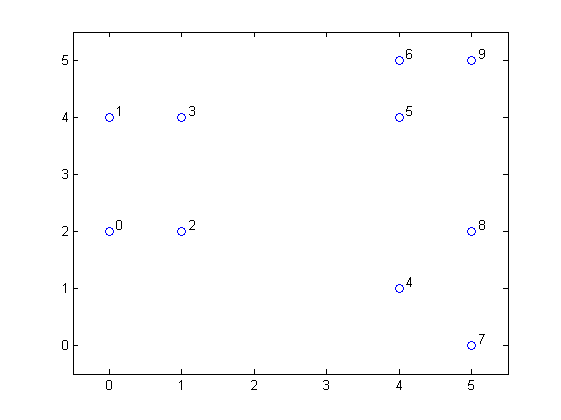
\includegraphics[bb=0 0 561 420,scale=0.37]{tsp_prob.png}
\label{fig:tsp_prob}} &
\subfigure[Subtours from the initial solution to the \ac{TSP} example]{
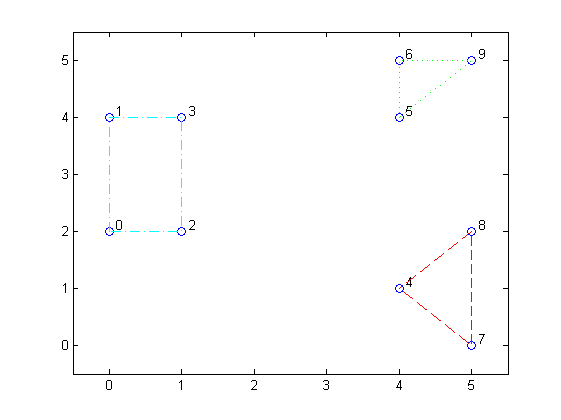
\includegraphics[bb=0 0 561 420,scale=0.37]{tsp_cuts1.png}
\label{fig:tsp_cuts1}}\\
\subfigure[Subtour from a later solution to the \ac{TSP} example]{
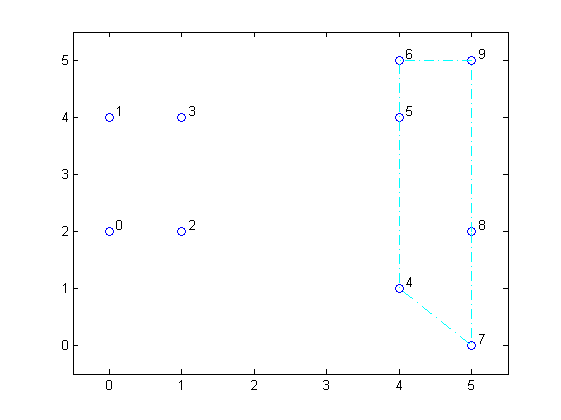
\includegraphics[bb=0 0 561 420,scale=0.37]{tsp_cuts2.png}
\label{fig:tsp_cuts2}} &
\subfigure[Final solution to the \ac{TSP} example]{
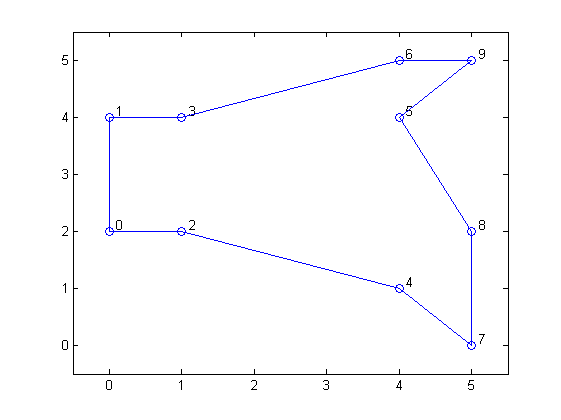
\includegraphics[bb=0 0 561 420,scale=0.37]{tsp_soln.png}
\label{fig:tsp_soln}}
\end{tabular}
\end{raggedright}
\caption{Cuts from an example \ac{TSP}} \label{fig:tsp}
\end{figure}

\begin{comment}
\subsection{Customised Cut Generation for the Wedding Planner problem} \label{sbs:wed_cuts}
\end{comment}

\subsection{Adding Customised Column Generation} \label{sbs:column}
Using Dippy it is easy to transform a problem into a form that can be solved by either branch and cut or branch, price and cut. Branch, price and cut decomposes a problem into a master problem and a number of distinct subproblems. We can identify subproblems using the \texttt{relaxation} member of the \texttt{DipProblem} class (remember the constraints restricting how patterns can be cut in \sbsref{sbs:sponge}). Once the subproblems have been identified, then they can either be ignored (when using branch and cut -- the default method for \ac{DIP}) or utilised (when using branch, price and cut -- specified by turning on the \texttt{doPriceCut} option).

\vfill
\newpage

In branch, price and cut, the original problem is decomposed into a master problem and multiple subproblems:
\begin{equation}
\begin{array}{rr@{\ }r@{\ }r@{\ }r@{\ }l}
             \min & c_1^\top x_1 & + \ c_2^\top x_2 & + \ \cdots & + \ c_k^\top x_k \\
\text{subject to} & A_1 x_1      & + \ A_2 x_2      & + \ \cdots & + \ A_k x_k      & = b \\
                  &              &   F_2 x_2      &          &                & = f_2 \\
                  &              &                &  \ddots  &                & \ \ \vdots \\
                  &              &                &          &   F_k x_k      & = f_k \\
                  & x_1 \in \mathbb{Z}^{+}_{n_1} &, x_2 \in \mathbb{Z}^{+}_{n_2}&, \ldots, x_k & \in \mathbb{Z}^{+}_{n_k} \quad
\end{array}
\label{eqn:decomp}
\end{equation}

Then, given a subset of extreme points for each subproblem, the \textit{restricted} master problem (RMP) finds an optimal solution and corresponding duals ($\pi$, $\gamma_1, \ldots, \gamma_k$):
\begin{equation}
\begin{array}{rr@{\ }r@{\ }r@{\ }r@{\ }ll}
             \min & c_1^\top x_1 & + \displaystyle\sum_{l_2=1}^{L_2} \left(c_2^\top y^2_{l_2} \right) \lambda^2_{l_2} & + \ \cdots & + \displaystyle\sum_{l_k=1}^{L_k} \left(c_k^\top y^k_{l_k} \right) \lambda^k_{l_k} \\
\text{subject to} & A_1 x_1      & + \displaystyle\sum_{l_2=1}^{L_2} \left(A_2 y^2_{l_2} \right) \lambda^2_{l_2} & + \ \cdots & + \displaystyle\sum_{l_k=1}^{L_k} \left( A_k y^k_{l_k} \right) \lambda^k_{l_k}      & = b & : \pi \\
                  &              &   \displaystyle\sum_{l_2=1}^{L_2} \lambda^2_{l_2}      &          &                & = 1 & : \gamma_1 \\
                  &              &                &  \ddots  &                & \ \ \vdots \\
                  &              &                &          &   \displaystyle\sum_{l_k=1}^{L_k} \lambda^k_{l_k}      & = 1 & : \gamma_k \\
                  &          x_1 & \in \mathbb{Z}^{+}_{n_1}, \lambda^2 \in \{0, 1\}_{L_2}, & \ldots, \lambda^k & \in \{0, 1\}_{L_k} \hspace{1.25cm} &
\end{array}
\label{eqn:rmp}
\end{equation}

New extreme points (columns for the RMP) are found by solving the subproblems ${\cal S}_j, j = 1, \ldots, k$ with the objective of minimising the reduced cost of a column in the RMP:
\begin{equation}
\begin{array}{rrl}
{\cal S}_j: \min & (c_j - \pi^\top A_j)^\top x_j + \gamma_j \\
\text{subject to} & F_j x_j      & = f_j \\
                  & x_j \in \mathbb{Z}^{+}_{n_j}
\end{array}
\label{eqn:subprob}
\end{equation}
If the objective value of ${\cal S}_j$ is $< 0$, then the column will improve the objective value of the RMP and is added.

The subproblems can either be solved using the default \ac{MILP} solver (Cbc) or a customised solver. A customised solver can be defined by the \texttt{relaxed\_solver} function. This function has 4 inputs:
\begin{enumerate}
\item \texttt{prob} -- the \texttt{DipProblem} being solved;
\item \texttt{index} -- the index $j$ of the subproblem being solved;
\item \texttt{redCosts} -- $c_j - \pi^\top A_j$, the reduced costs for the $x_j$ variables;
\item \texttt{convexDual} -- $\gamma_j$, the dual value for the convexity constraint for this subproblem.
\end{enumerate}
In addition to subproblem solutions using dual values, initial columns for subproblems can also be generated either automatically using Cbc or using a customised approach. A customised approach to initial variable generation can be defined by the \texttt{init\_vars} function. This function has only 1 input, \texttt{prob}, the \texttt{DipProblem} being solved.

\subsection{Customised Column Generation for the Capacitated Facility Location problem} \label{sbs:fac_cols}

Starting from the original capacitated facility location problem (see \sbsref{sbs:facility}), we can define subproblems for each facility location that define the capacity constraints at that location:
\lstinputlisting[firstnumber=35,linerange=35-44]{C:/COIN/Dippy/examples/facility_decomp.py}

All remaining constraints (the assignment constraints - ensuring each product is assigned to a facility) form the master problem when using branch, price and cut. To use branch, price and cut we turn on the \texttt{doPricCut} option:
\lstinputlisting[firstnumber=162,linerange=162-166]{C:/COIN/Dippy/examples/facility_decomp.py}

Note that symmetry is also present in the decomposed problem, so we add the ordering constraints to the RMP (see \sbsref{sbs:fac_brch}):
\lstinputlisting[firstnumber=46,linerange=46-49]{C:/COIN/Dippy/examples/facility_decomp.py}

In branch, price and cut, the RMP requires 10.39s of CPU times and creates a tree with 27 nodes (compared with 0.28s and 76 nodes for the original branch and cut approach with ordering constraints). Note that the \texttt{generateInitVars} option uses Cbc by default to find initial columns for the RMP and then Cbc is also used (by default) to solve the subproblems that generate facilities at locations along with products produced at that facility. However, we may be able to speed up the overall solution process by providing our own approaches to solving the pricing subproblems and generating initial variables.

In the pricing subproblem, we are looking to assign products to a facility in order to provide negative reduced cost. Producing a product at a facility provides the reduced cost of $x_{ij}$ (\texttt{assign\_vars[(i, j)]}), but will decrease the wasted capacity and hence reduce the contribution of the reduced cost of $w_i$ (\texttt{waste\_vars[i]}). Here, we calculate the total contribution to reduced cost of adding an item (= reduced cost of $x_{ij} -$ reduced cost of $w_i \times r_j$) and then calculate an items efficiency by dividing this contribution by its weight. Then, we build a minimum reduced cost facility by using a greedy algorithm to choose items in order of best efficiency. Since we can access the problem data, variables and their reduced cost, this is straightforward to implement in Dippy:
\lstinputlisting[firstnumber=69,linerange=69-105]{C:/COIN/Dippy/examples/facility_decomp.py}

Adding this customised solver reduces the solution time to 1.61s of CPU time and the search tree to 7 nodes.

To generate initial facilities (complete with assigned products) we implemented two approaches. The first approach used a first-fit approach and considered the products in order of decreasing requirement:
\lstinputlisting[firstnumber=107,linerange=107-138]{C:/COIN/Dippy/examples/facility_decomp.py}

The second approach simply assigned one product to each facility:
\lstinputlisting[firstnumber=140,linerange=140-153]{C:/COIN/Dippy/examples/facility_decomp.py}

\newpage

Using Dippy we can define both approaches at once and then define which one to use by setting the \texttt{init\_vars} method:
\lstinputlisting[firstnumber=155,linerange=155-156]{C:/COIN/Dippy/examples/facility_decomp.py}

The effects of column generation, included a customised subproblem solver and initial variable generator are shown in \scnref{scn:concl}.

\subsection{Customised Column Generation for the Cutting Stock problem} \label{sbs:cut_cols}

For the Sponge Roll Production problem (see \sbsref{sbs:sponge}), the subproblem consists of the cutting pattern constraint:
\lstinputlisting[firstnumber=55,linerange=55-59]{C:/COIN/Dippy/examples/cutting_stock.py}

To generate cutting patterns with negative reduced cost in the customised \texttt{relaxed\_solver} function, we first set ``profit'' coefficients to be $-$ reduced cost and ``size'' coefficients to be the length of the required items:
\lstinputlisting[firstnumber=62,linerange=62-68]{C:/COIN/Dippy/examples/cutting_stock.py}

Then, we use \ac{DP} to find a maximum profit knapsack. The \ac{DP} recursion is:
\[\begin{array}{rcl}
I &=& \text{set of possible items to include}; \\
W &=& \text{capacity of knapsack}; \\
w_i &=& \text{``size'' of item } i; \\
p_i &=& \text{``profit'' of including item} i; \\
V(I, W) &=& \text{maximum profit when considering items from $I$} \\
& &\text{for inclusion in a knapsack of capacity $W$} \\
V(\emptyset, W) &=& 0 \\
V(I, 0) &=& 0 \\
V(I, W) &=& \max\big[\underset{\text{\begin{tabular}{c}don't include any \\[-3pt] item, consider \\[-3pt] smaller knapsack \end{tabular}}}{\underbrace{V(I, W - 1)}}, \max_{i \in I} \underset{\text{include item $i$}}{\underbrace{p_i + V(I, W - w_i)}} \big].
\end{array}\]

\newpage

The \texttt{kp} function implements the \ac{DP} recursion:
\lstinputlisting[firstnumber=97,linerange=97-122]{C:/COIN/Dippy/examples/cutting_stock.py}

The customised \texttt{relaxed\_solver} function calls \texttt{kp} to find the maximum profit (= most negative reduced cost) cutting pattern:
\lstinputlisting[firstnumber=70,linerange=70-70]{C:/COIN/Dippy/examples/cutting_stock.py}
checks it is valid and adds it to the restricted master problem if the total reduced cost is negative (cutting pattern reduced cost + pattern use reduced cost $-$ convexity constraint dual $< 0$).
\lstinputlisting[firstnumber=79,linerange=79-93]{C:/COIN/Dippy/examples/cutting_stock.py}

The effect of the customised subproblem solver is a reduction from 33.31s to 28.30s of CPU time and 175 to 131 nodes.

\begin{comment}
\subsection{Customised Column Generation for the Wedding Planner problem} \label{sbs:wed_cols}
\end{comment}

\newpage\subsection{Adding Customised Heuristics} \label{sbs:heuristics}
To add user-defined heuristics in Dippy, we first define a new procedure for node heuristics, \texttt{heuristics}. This function has three inputs:
\begin{enumerate}
\item \texttt{prob} -- the \texttt{DipProblem} being solved;
\item \texttt{xhat} -- an indexable object representing the fraction solution at the current node;
\item \texttt{cost} -- the objective coefficients of the variables.
\end{enumerate}
Multiple heuristics can be executed and all heuristic solutions can be returned to \ac{DIP}. Different problems benefit from different heuristic approaches and a heuristic that solves the original problem may not be as useful when a fractional solution is available. We show how solve a heuristic for the overall problem and also how to implement a heuristic for fractional solutions. As in \scnref{scn:branch}, Python's scoping rules allow us to easily access the solution values of variables in our problem.

\subsection{Customised Heuristics for the Capacitated Facility Location problem} \label{sbs:fac_heur}

An initial allocation of production to locations can be found heuristically using the same first-fit heuristic that provided initial solutions for the column generation approach (see \sbsref{sbs:fac_cols}). The first-fit heuristic iterates through the items requiring production and the facility locations allocating production at the first facility that has sufficient capacity to produce the item.
\lstinputlisting[firstnumber=116,linerange=116-127]{C:/COIN/Dippy/examples/facility.py}

\vfill
\newpage
\lstinputlisting[firstnumber=129,linerange=129-144]{C:/COIN/Dippy/examples/facility.py}

The first-fit heuristic can then be used to provide an initial, feasible solution at the root node within the customised \texttt{heuristics} function (see lines 215-220):
\lstinputlisting[firstnumber=211,linerange=211-230]{C:/COIN/Dippy/examples/facility.py}

Running the first-fit heuristic before starting the branching process increases the solution time from 1.17s to 1.48s of CPU time and the number of nodes in the search tree from 375 nodes to 399 nodes.

\newpage

At each node in the branch-and-bound tree, the fractional solution (provided by \texttt{xhat}) gives an indication of the best allocation of production, albeit fractional. One heuristic approach to ``fixing'' the fractional solution is to consider each allocation (of an item's production to a facility) in order of decreasing fractionality and use a first-fit approach:
\lstinputlisting[firstnumber=146,linerange=146-192]{C:/COIN/Dippy/examples/facility.py}
\newpage
\lstinputlisting[firstnumber=194,linerange=194-209]{C:/COIN/Dippy/examples/facility.py}

The first-fit approach that is guided by fractional values can then be used within the \texttt{heuristics} function (see lines 225-229 in the previous listing) to create integer solutions from fractional solutions at each node.

Adding the first-fit heuristic guided by fractional values increases the solution time further from 1.48s to 1.89s of CPU time and the number of nodes remains at 399.

The reason this heuristic (in fact any heuristic) was not that helpful for this problem is that:
\begin{itemize}
\item the optimal solution is found within the first 10 nodes without any heuristics, so the heuristic only provides an improved upper bound for $< 10$ nodes;
\item the extra overhead of the heuristic at each node increases the solution time and the heuristic affects the search procedure in a way that more nodes are explored.
\end{itemize}

Heuristics generally only help in problems where feasibility is more difficult by providing upper bounds when ``fixing'' fractional solutions. In this problem, the optimal solution is found quickly and the rest of the search tree checks solutions that are symmetric.

In \scnref{scn:concl} we show the effect of the heuristic when symmetry is removed.

\begin{comment}
\subsection{Customised Heuristics for the Wedding Planner problem} \label{sbs:wed_heur}
\end{comment}

\subsection{Combining Techniques} \label{sbs:combine}

\begin{table}[ht]
%\begin{minipage}[c]{\textwidth}
%\begin{small}
\begin{center}
\begin{tabular}[c]{|lll|}
\hline
\textbf{Strategies}																 & \textbf{Time (s)}	& \textbf{Nodes} \\ 
\hline & &\\[-10pt]
Default (branch and cut)                           & 0.26							  & 419 \\
\hline
+ ordering constraints (OC)                        & 0.05 							& 77 \\
+ OC \& advanced branching (AB)                    & 0.01 							& 3 \\
\hline
+ weighted inequalities (WI)                       & 0.34 							& 77 \\
+ WI \& OC                                         & 0.17 							& 20 \\
+ WI \& OC \& AB                                   & 0.06 							& 4 \\
\hline
+ first-fit heuristic (FF) at root node            & 0.28 							& 419 \\
+ FF \& OC                                         & 0.05 							& 77 \\
+ FF \& OC \& AB                                   & 0.01 							& 3 \\
\hline
+ FF \& WI                                         & 0.36 							& 77 \\
+ FF \& WI \& OC                                   & 0.14 							& 17 \\
+ FF \& WI \& OC \& AB                             & 0.05 							& 3 \\
\hline
+ fractional-fit heuristic (RF) at nodes           & 0.28 							& 419 \\
+ RF \& OC                                         & 0.05 							& 77 \\
+ RF \& OC \& AB                                   & 0.01 							& 3 \\
\hline
+ WI \& RF                                         & 0.38 							& 77 \\
+ WI \& RF \& OC                                   & 0.14 							& 17 \\
+ WI \& RF \& OC \& AB                             & 0.05 							& 3 \\
\hline
+ FF \& RF                                         & 0.28 							& 419 \\
+ FF \& RF \& OC                                   & 0.05 							& 77 \\
+ FF \& RF \& OC \& AB                             & 0.01 							& 3 \\
\hline
+ WI \& FF \& RF                                   & 0.38 							& 77 \\
+ WI \& FF \& RF \& OC                             & 0.14 							& 17 \\
+ WI \& FF \& RF \& OC \& AB                       & 0.05 							& 3 \\
\hline
+ column generation (CG)                           & 2.98 							& 37 \\
+ CG \& OC                                         & 2.07 							& 23 \\
+ CG \& OC \& AB                                   & 0.56								& 10 \\
\hline
+ CG \& customised subproblem solver (CS)          & 2.87 							& 37 \\
+ CG \& CS \& OC                                   & 1.95 							& 23 \\
+ CG \& CS \& OC \& AB                             & 0.44 							& 10 \\
\hline
+ CG \& first-fit initial variable generation (FV) & 3.96 							& 45 \\
+ CG \& CS \& FV                                   & 3.72 							& 45 \\
+ CG \& CS \& FV \& OC                             & 1.70 							& 18 \\
+ CG \& CS \& FV \& OC \& AB                       & 0.22 							& 3\\
\hline
+ CG \& one-each initial variable generation (OV)  & 3.40 							& 41 \\
+ CG \& CS \& OV                                   & 3.33 							& 41 \\
+ CG \& CS \& OV \& OC                             & 2.23 							& 24 \\
+ CG \& CS \& OV \& OC \& AB                       & 0.27 							& 3 \\
\hline
\end{tabular} 
\end{center}
%\end{small}
%\end{minipage}
\caption{Experiments for the Capacitated Facility Location Problem} \label{tab:fac_exp}
\end{table}

The techniques and modifications of the solver framework can be combined to improve performance further.
\Tabref{tab:fac_exp} shows that it is possible to quickly and easily test many approaches for a particular problem, including combinations of approaches\footnote{All tests were run using Python 2.7.1 on a Windows~7 machine with an Intel Core~2~Duo T9500@2.60GHz CPU.}.
Looking at the results shows that the heuristics only help when the size of the branch-and-bound tree has been reduced with other approaches, such as ordering constraints and advanced branching.
Approaches for solving this problem that warrant further investigation use column generation, the customised solver and either ordering constraints or the first-fit heuristic to generate initial variables.
Tests with different data showed that the solution time for branch-price-and-cut doesn't increase with problem size as quickly as for branch-and-cut, so the column generation approaches are worth considering for larger problems.
